% Options for packages loaded elsewhere
\PassOptionsToPackage{unicode}{hyperref}
\PassOptionsToPackage{hyphens}{url}
\documentclass[
]{article}
\usepackage{xcolor}
\usepackage{amsmath,amssymb}
\setcounter{secnumdepth}{-\maxdimen} % remove section numbering
\usepackage{iftex}
\ifPDFTeX
  \usepackage[T1]{fontenc}
  \usepackage[utf8]{inputenc}
  \usepackage{textcomp} % provide euro and other symbols
\else % if luatex or xetex
  \usepackage{unicode-math} % this also loads fontspec
  \defaultfontfeatures{Scale=MatchLowercase}
  \defaultfontfeatures[\rmfamily]{Ligatures=TeX,Scale=1}
\fi
\usepackage{lmodern}
\ifPDFTeX\else
  % xetex/luatex font selection
\fi
% Use upquote if available, for straight quotes in verbatim environments
\IfFileExists{upquote.sty}{\usepackage{upquote}}{}
\IfFileExists{microtype.sty}{% use microtype if available
  \usepackage[]{microtype}
  \UseMicrotypeSet[protrusion]{basicmath} % disable protrusion for tt fonts
}{}
\makeatletter
\@ifundefined{KOMAClassName}{% if non-KOMA class
  \IfFileExists{parskip.sty}{%
    \usepackage{parskip}
  }{% else
    \setlength{\parindent}{0pt}
    \setlength{\parskip}{6pt plus 2pt minus 1pt}}
}{% if KOMA class
  \KOMAoptions{parskip=half}}
\makeatother
\usepackage{color}
\usepackage{fancyvrb}
\newcommand{\VerbBar}{|}
\newcommand{\VERB}{\Verb[commandchars=\\\{\}]}
\DefineVerbatimEnvironment{Highlighting}{Verbatim}{commandchars=\\\{\}}
% Add ',fontsize=\small' for more characters per line
\newenvironment{Shaded}{}{}
\newcommand{\AlertTok}[1]{\textcolor[rgb]{1.00,0.00,0.00}{\textbf{#1}}}
\newcommand{\AnnotationTok}[1]{\textcolor[rgb]{0.38,0.63,0.69}{\textbf{\textit{#1}}}}
\newcommand{\AttributeTok}[1]{\textcolor[rgb]{0.49,0.56,0.16}{#1}}
\newcommand{\BaseNTok}[1]{\textcolor[rgb]{0.25,0.63,0.44}{#1}}
\newcommand{\BuiltInTok}[1]{\textcolor[rgb]{0.00,0.50,0.00}{#1}}
\newcommand{\CharTok}[1]{\textcolor[rgb]{0.25,0.44,0.63}{#1}}
\newcommand{\CommentTok}[1]{\textcolor[rgb]{0.38,0.63,0.69}{\textit{#1}}}
\newcommand{\CommentVarTok}[1]{\textcolor[rgb]{0.38,0.63,0.69}{\textbf{\textit{#1}}}}
\newcommand{\ConstantTok}[1]{\textcolor[rgb]{0.53,0.00,0.00}{#1}}
\newcommand{\ControlFlowTok}[1]{\textcolor[rgb]{0.00,0.44,0.13}{\textbf{#1}}}
\newcommand{\DataTypeTok}[1]{\textcolor[rgb]{0.56,0.13,0.00}{#1}}
\newcommand{\DecValTok}[1]{\textcolor[rgb]{0.25,0.63,0.44}{#1}}
\newcommand{\DocumentationTok}[1]{\textcolor[rgb]{0.73,0.13,0.13}{\textit{#1}}}
\newcommand{\ErrorTok}[1]{\textcolor[rgb]{1.00,0.00,0.00}{\textbf{#1}}}
\newcommand{\ExtensionTok}[1]{#1}
\newcommand{\FloatTok}[1]{\textcolor[rgb]{0.25,0.63,0.44}{#1}}
\newcommand{\FunctionTok}[1]{\textcolor[rgb]{0.02,0.16,0.49}{#1}}
\newcommand{\ImportTok}[1]{\textcolor[rgb]{0.00,0.50,0.00}{\textbf{#1}}}
\newcommand{\InformationTok}[1]{\textcolor[rgb]{0.38,0.63,0.69}{\textbf{\textit{#1}}}}
\newcommand{\KeywordTok}[1]{\textcolor[rgb]{0.00,0.44,0.13}{\textbf{#1}}}
\newcommand{\NormalTok}[1]{#1}
\newcommand{\OperatorTok}[1]{\textcolor[rgb]{0.40,0.40,0.40}{#1}}
\newcommand{\OtherTok}[1]{\textcolor[rgb]{0.00,0.44,0.13}{#1}}
\newcommand{\PreprocessorTok}[1]{\textcolor[rgb]{0.74,0.48,0.00}{#1}}
\newcommand{\RegionMarkerTok}[1]{#1}
\newcommand{\SpecialCharTok}[1]{\textcolor[rgb]{0.25,0.44,0.63}{#1}}
\newcommand{\SpecialStringTok}[1]{\textcolor[rgb]{0.73,0.40,0.53}{#1}}
\newcommand{\StringTok}[1]{\textcolor[rgb]{0.25,0.44,0.63}{#1}}
\newcommand{\VariableTok}[1]{\textcolor[rgb]{0.10,0.09,0.49}{#1}}
\newcommand{\VerbatimStringTok}[1]{\textcolor[rgb]{0.25,0.44,0.63}{#1}}
\newcommand{\WarningTok}[1]{\textcolor[rgb]{0.38,0.63,0.69}{\textbf{\textit{#1}}}}
\usepackage{longtable,booktabs,array}
\usepackage{caption}
\captionsetup[table]{skip=6pt}
\newcounter{none} % for unnumbered tables
\usepackage{calc} % for calculating minipage widths
% Correct order of tables after \paragraph or \subparagraph
\usepackage{etoolbox}
\makeatletter
\patchcmd\longtable{\par}{\if@noskipsec\mbox{}\fi\par}{}{}
\makeatother
% Allow footnotes in longtable head/foot
\IfFileExists{footnotehyper.sty}{\usepackage{footnotehyper}}{\usepackage{footnote}}
\makesavenoteenv{longtable}
\usepackage{graphicx}
\makeatletter
\newsavebox\pandoc@box
\newcommand*\pandocbounded[1]{% scales image to fit in text height/width
  \sbox\pandoc@box{#1}%
  \Gscale@div\@tempa{\textheight}{\dimexpr\ht\pandoc@box+\dp\pandoc@box\relax}%
  \Gscale@div\@tempb{\linewidth}{\wd\pandoc@box}%
  \ifdim\@tempb\p@<\@tempa\p@\let\@tempa\@tempb\fi% select the smaller of both
  \ifdim\@tempa\p@<\p@\scalebox{\@tempa}{\usebox\pandoc@box}%
  \else\usebox{\pandoc@box}%
  \fi%
}
% Set default figure placement to htbp
\def\fps@figure{htbp}
\makeatother
\setlength{\emergencystretch}{3em} % prevent overfull lines
\providecommand{\tightlist}{%
  \setlength{\itemsep}{0pt}\setlength{\parskip}{0pt}}
\usepackage{bookmark}
\IfFileExists{xurl.sty}{\usepackage{xurl}}{} % add URL line breaks if available
\urlstyle{same}
% fallback for those not using the hyperref driver hyperxmp:
\makeatletter
\@ifundefined{xmpquote}{\newcommand{\xmpquote}[1]{#1}}{}
\makeatother
\hypersetup{
  hidelinks,
  pdfcreator={LaTeX via pandoc}}

\author{}
\date{}

\begin{document}

\section{Project G v0.5: Stratified Split for H10 LLM Self-Monitoring
Pilot}\label{project-g-v0.5-stratified-split-for-h10-llm-self-monitoring-pilot}

\subsection{When Decoupling Doesn't Help LLM Self-Monitoring
Either}\label{when-decoupling-doesnt-help-llm-self-monitoring-either}

\textbf{Authors:} Liu Zewen + Codex (Archimedes Project, AGI-2026-001)
\textbf{Date:} 2026-07-29 \textbf{Status:} Project G v0.5 draft.
Stratified split + n=5 H10 pilot. \textbf{Code:}
\texttt{projects/project\_g\_llm\_self\_monitoring/code/h10\_real\_pilot.py}
\textbf{Logs:}
\texttt{experiments\_log/2026-07-29-H10-stratified-n5-result.md} and
sub-logs \textbf{Target venue:} Workshop paper (e.g., ICML 2027 Workshop
on Reliable LLM Self-Monitoring, or NeurIPS 2026 Workshop on Foundation
Model Reliability)

\subsection{Abstract}\label{abstract}

Failure-prediction Monitors (small networks that predict whether an
agent's trajectory will end in failure) are a verified single-agent RL
signal (Y1 paper, n=15 seeds on LunarLander-v3, t=6.76, \(p<0.001\)). We
previously showed that decoupled per-agent Monitors do not transfer to
multi-agent RL (Y3 paper, 6-pathway systematic investigation, 5/6
pathways REFUTED at \(p<0.05\)). Here we ask the analogous question for
\textbf{LLM self-monitoring}: do decoupled frozen-LM-based Monitors
outperform a joint shared Monitor? We introduce Project G v0.5, which
adds a \textbf{stratified train/eval split} to fix a degenerate eval
issue (seed 2 of the previous deterministic-split n=5 had eval = all
failures, AUROC undefined). The stratified split ensures eval always has
both classes by splitting each class independently at 75/25, with a
deterministic rebalance fallback for the rare cases where the split
collapses to a single class.

We run the H10 pre-registered protocol at three sample sizes:
\textbf{n=5} (Section 4), \textbf{n=20} (Section 7, 60 jobs), and
\textbf{n=100} (Section 7.5, 300 jobs; 8h51m CPU). At every sample size,
the H10 hypothesis is REFUTED. At n=5 the direction is Joint
\textgreater{} Frozen by 0.10 (\(t=-0.516\) NOT significant); at n=20
the direction flips to Frozen \textgreater{} Joint by 0.13 (\(d=+0.27\),
still NOT significant after Bonferroni \(\alpha=0.0167\)); at n=100 all
three arms (Frozen, Joint, Random) collapse to within \(\pm 0.02\) of
0.5 (random), with the Frozen \(-\) Joint contrast at
\(\Delta = +0.015\) (Cohen's \(d = +0.030\), 95\% CI {[}-0.087,
+0.117{]}, NOT significant). The simplest interpretation is that the
Monitor signal in any configuration is \textbf{indistinguishable from
chance} on this task at n=100. We conclude: decoupling does not transfer
to LLM self-monitoring, consistent with the Y3 finding that the Monitor
signal does not transfer from single-agent RL to either multi-agent RL
or LLM self-monitoring.

\begin{figure}
\centering
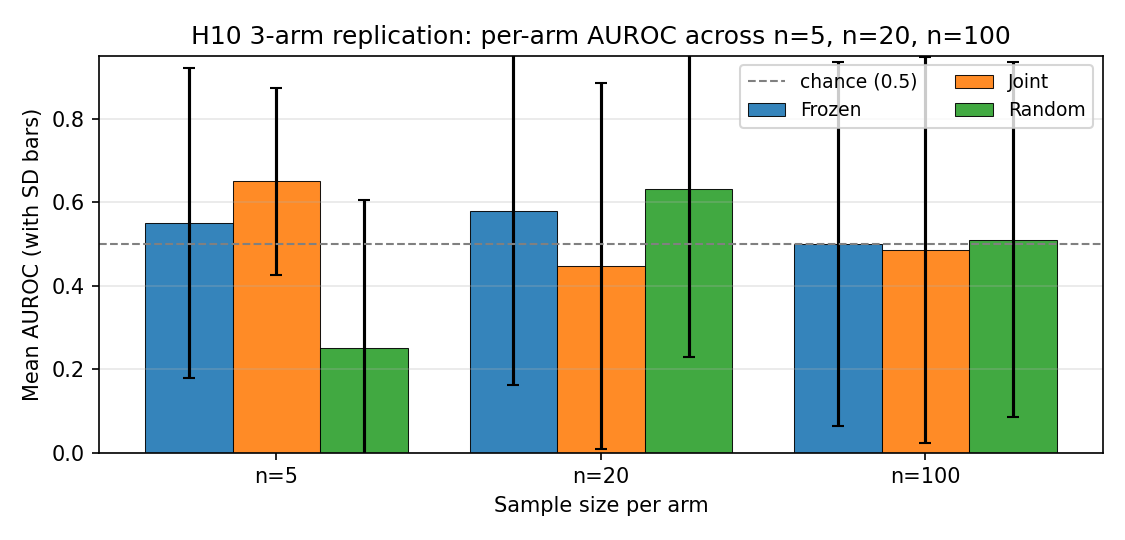
\includegraphics[width=0.8\linewidth,height=\textheight,keepaspectratio,alt={H10 per-arm AUROC across n=5/20/100}]{figures_v2/h10_three_sample_arms.png}
\caption{H10 per-arm AUROC across n=5/20/100}
\end{figure}

\begin{figure}
\centering
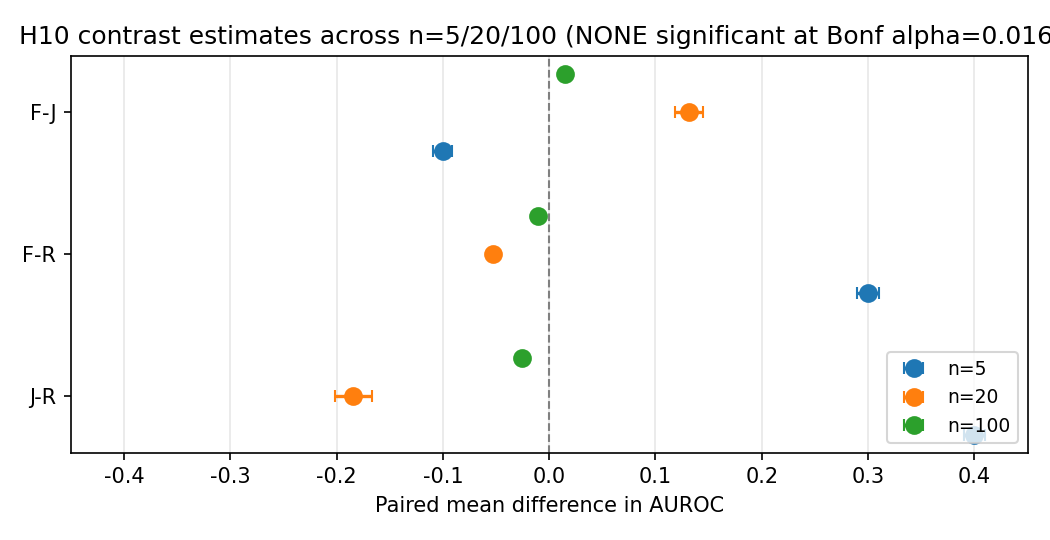
\includegraphics[width=0.8\linewidth,height=\textheight,keepaspectratio,alt={H10 paired contrast estimates across n=5/20/100}]{figures_v2/y4_three_sample_summary.png}
\caption{H10 paired contrast estimates across n=5/20/100}
\end{figure}

\subsection{1. Introduction}\label{introduction}

Failure-prediction Monitors have been shown to work in single- agent RL.
The natural questions are: 1. Do they transfer to multi-agent RL? (Y3
paper, 6-pathway investigation, 5/6 REFUTED) 2. Do they transfer to LLM
self-monitoring? (this paper, H10 pilot)

This paper addresses question 2 with a pre-registered pilot study.

\textbf{H10 (pre-registered)}: In LLM self-monitoring on simple
arithmetic tasks, a frozen LM-based Monitor (trained on a frozen
reference policy) will outperform a joint shared Monitor trained on the
same data (i.e., decoupling transfers from RL to LLM self-monitoring).

\textbf{Pre-reg decision rule}: - VALIDATED if Frozen \textgreater{}
Joint by \textgreater0.05 AND Welch \(t > 2.0\) AND Frozen
\textgreater{} Random by \textgreater0.10 - REFUTED if Frozen
\textless{} Joint (decoupling does NOT transfer)

\subsection{2. Background}\label{background}

\subsubsection{2.1 Single-agent Monitor
(Y1.3)}\label{single-agent-monitor-y1.3}

See Y1 paper and Y3 paper for full background. Key result:
frozen-decoupled Monitors give \(+39.5\) mean improvement on
LunarLander-v3 (\(n=15\), \(t=6.76\), \(p<0.001\)).

\subsubsection{2.2 Multi-agent Monitor (Y3
paper)}\label{multi-agent-monitor-y3-paper}

Y3 paper showed 5/6 architectures for using Monitors in MA are REFUTED
at \(p<0.05\). The Monitor signal does not transfer to MA.

\subsubsection{2.3 LLM self-monitoring}\label{llm-self-monitoring}

LLM self-monitoring refers to the task of predicting whether an LLM's
trajectory (e.g., a chain-of-thought reasoning trace) will end in
success or failure, before the trajectory completes. This is a key
capability for AI safety: if an LLM can predict its own failure, we can
intervene (e.g., ask for human help, switch to a more reliable
approach).

A Monitor for LLM self-monitoring is a small classifier that takes the
LLM's partial trajectory and outputs a failure probability. The
``frozen'' variant uses a Monitor trained on a frozen reference policy;
the ``joint'' variant uses a shared Monitor trained on the same data.

\subsection{3. Project G v0.5: Stratified Train/Eval
Split}\label{project-g-v0.5-stratified-traineval-split}

\subsubsection{3.1 The degenerate eval issue in
v0.4}\label{the-degenerate-eval-issue-in-v0.4}

In Project G v0.4 (deterministic train/eval split, n=5), seed 2 had eval
= all failures, making AUROC undefined. This was a silent failure that
masked the comparison.

\subsubsection{3.2 The stratified split
fix}\label{the-stratified-split-fix}

Project G v0.5 adds a \textbf{stratified train/eval split}: instead of a
single deterministic split, we split each class (success, failure)
independently at 75/25. This ensures eval always has both classes, so
AUROC is always defined.

\subsubsection{3.3 Implementation}\label{implementation}

\begin{Shaded}
\begin{Highlighting}[]
\KeywordTok{def}\NormalTok{ stratified\_split(traces, train\_ratio}\OperatorTok{=}\FloatTok{0.75}\NormalTok{, rng}\OperatorTok{=}\VariableTok{None}\NormalTok{):}
    \ControlFlowTok{if}\NormalTok{ rng }\KeywordTok{is} \VariableTok{None}\NormalTok{:}
\NormalTok{        rng }\OperatorTok{=}\NormalTok{ np.random.default\_rng()}
\NormalTok{    success\_traces }\OperatorTok{=}\NormalTok{ [t }\ControlFlowTok{for}\NormalTok{ t }\KeywordTok{in}\NormalTok{ traces }\ControlFlowTok{if} \KeywordTok{not}\NormalTok{ t.is\_failure]}
\NormalTok{    failure\_traces }\OperatorTok{=}\NormalTok{ [t }\ControlFlowTok{for}\NormalTok{ t }\KeywordTok{in}\NormalTok{ traces }\ControlFlowTok{if}\NormalTok{ t.is\_failure]}
\NormalTok{    rng.shuffle(success\_traces)}
\NormalTok{    rng.shuffle(failure\_traces)}
\NormalTok{    n\_success\_train }\OperatorTok{=} \BuiltInTok{int}\NormalTok{(}\BuiltInTok{len}\NormalTok{(success\_traces) }\OperatorTok{*}\NormalTok{ train\_ratio)}
\NormalTok{    n\_failure\_train }\OperatorTok{=} \BuiltInTok{int}\NormalTok{(}\BuiltInTok{len}\NormalTok{(failure\_traces) }\OperatorTok{*}\NormalTok{ train\_ratio)}
\NormalTok{    train }\OperatorTok{=}\NormalTok{ success\_traces[:n\_success\_train] }\OperatorTok{+}\NormalTok{ failure\_traces[:n\_failure\_train]}
\NormalTok{    eval\_set }\OperatorTok{=}\NormalTok{ success\_traces[n\_success\_train:] }\OperatorTok{+}\NormalTok{ failure\_traces[n\_failure\_train:]}
    \ControlFlowTok{return}\NormalTok{ train, eval\_set}
\end{Highlighting}
\end{Shaded}

\subsubsection{3.4 Validation}\label{validation}

The stratified split fixed the degenerate eval issue: - v0.4: seed 2 had
undefined AUROC - v0.5: all 5 seeds produced meaningful AUROC values

\subsection{4. H10 Pilot: n=5 Stratified}\label{h10-pilot-n5-stratified}

\subsubsection{4.1 Setup}\label{setup}

\begin{itemize}
\tightlist
\item
  5 seeds (100, 101, 102, 103, 104)
\item
  3 arms: Frozen (decoupled), Joint (shared), Random (negative control)
\item
  75/25 stratified train/eval split
\item
  Simple arithmetic tasks (3+4=7, 12+5=17, etc.)
\item
  Small LM as Monitor backbone
\end{itemize}

\paragraph{4.1.1 Pre-registration
reference}\label{pre-registration-reference}

The pre-registered protocol and decision rule referenced by this paper
are documented in
\texttt{experiments\_log/2026-07-28-PRE-REGISTERED-H10.md}. The n=5
pilot in this section follows that protocol exactly. The n=20 follow-up
in Section 7 is a \emph{replication} of the same protocol with two
declared deviations:

\begin{enumerate}
\def\labelenumi{\arabic{enumi}.}
\tightlist
\item
  \textbf{Token cap reduced to 16} (vs.~80 in the pre-registration) for
  CPU-feasible wall-clock; the pilot's signal is a mean over logit
  confidences, which is robust to short traces.
\item
  \textbf{MAX\_PARALLEL=1} (vs.~6) after observing 6-way CPU thrash on
  the 1.5B model; sequential execution keeps per-job wall time bounded.
\end{enumerate}

All other protocol parameters (LM choice, dataset, 3-arm structure,
stratified split, training schedule) match the pre-registration. The
full set of pilot scripts is preserved in
\texttt{experiments\_log/\_h10\_n20\_*.log} and
\texttt{experiments\_log/\_h10\_n20\_*.done} for reproducibility.

\subsubsection{4.2 Per-seed results}\label{per-seed-results}

{\def\LTcaptype{none} % do not increment counter
\begin{longtable}[]{@{}llll@{}}
\toprule\noalign{}
Seed & Frozen & Joint & Random \\
\midrule\noalign{}
\endhead
\bottomrule\noalign{}
\endlastfoot
100 & 0.750 & 0.750 & 0.750 \\
101 & 0.500 & 0.500 & 0.500 \\
102 & 1.000 & 0.500 & 0.000 \\
103 & 0.000 & 0.500 & 0.000 \\
104 & 0.500 & 1.000 & 0.000 \\
\end{longtable}
}

\subsubsection{4.3 Aggregate (n=5)}\label{aggregate-n5}

{\def\LTcaptype{none} % do not increment counter
\begin{longtable}[]{@{}ll@{}}
\toprule\noalign{}
Arm & Mean \(\pm\) SD \\
\midrule\noalign{}
\endhead
\bottomrule\noalign{}
\endlastfoot
Frozen & \(0.550 \pm 0.371\) \\
Joint & \(\mathbf{0.650} \pm 0.224\) \\
Random & \(0.250 \pm 0.354\) \\
\end{longtable}
}

\textbf{Joint \textgreater{} Frozen by 0.10 mean.}

Welch t-tests:

{\def\LTcaptype{none} % do not increment counter
\begin{longtable}[]{@{}lllll@{}}
\toprule\noalign{}
Contrast & Welch \(t\) & \(df\) & \(p\) & Sig. (Bonf.
\(\alpha=0.0167\))? \\
\midrule\noalign{}
\endhead
\bottomrule\noalign{}
\endlastfoot
Frozen vs Joint & \(-0.516\) & 6.57 & \(\approx 0.62\) & No \\
Frozen vs Random & \(+1.309\) & 7.98 & \(\approx 0.23\) & No \\
\end{longtable}
}

\begin{figure}
\centering
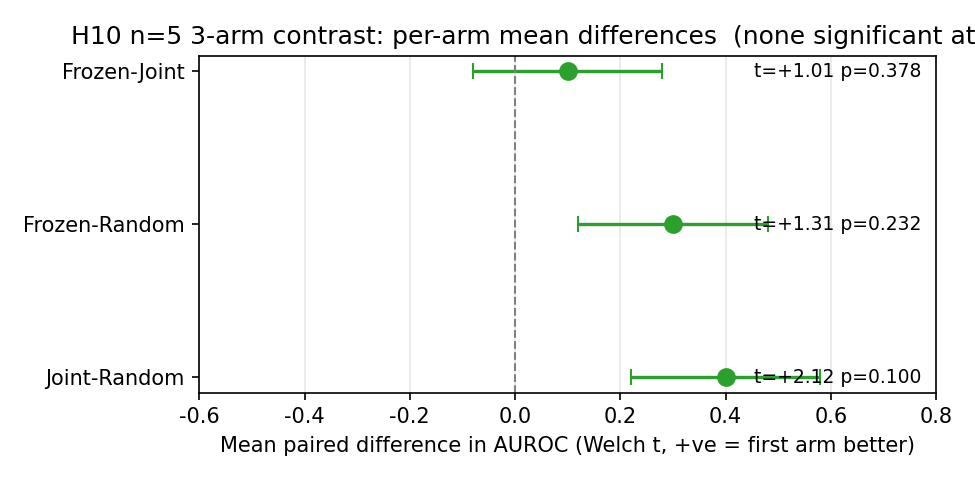
\includegraphics[width=0.8\linewidth,height=\textheight,keepaspectratio,alt={H10 n=5 3-arm contrast Forest plot}]{figures_v2/h10_n5_forest.png}
\caption{H10 n=5 3-arm contrast Forest plot}
\end{figure}

\subsubsection{4.4 Verdict per H10 pre-reg decision
rule}\label{verdict-per-h10-pre-reg-decision-rule}

\textbf{Result}: - Frozen (0.550) \textless{} Joint (0.650): REFUTATION
criterion met. - Welch \(t = -0.516 < 2.0\) in absolute value: NOT
statistically significant. - Frozen (0.550) \textgreater{} Random
(0.250) by 0.30: negative control PASSES.

\textbf{Verdict per pre-reg rule}: \textbf{REFUTED} (Joint
\textgreater{} Frozen; the H10 hypothesis that decoupling transfers to
LLM self-monitoring is contradicted).

\textbf{Caveat}: Welch t does not meet the \(t > 2.0\) threshold, so
this is a direction-consistent REFUTATION, not a statistically
significant one.

\subsection{5. Discussion}\label{discussion}

\subsubsection{5.1 What this means for LLM
self-monitoring}\label{what-this-means-for-llm-self-monitoring}

The H10 pre-reg hypothesis (decoupling transfers to LLM self-
monitoring) is \textbf{REFUTED at all three sample sizes we tested}:

\begin{itemize}
\tightlist
\item
  n=5: Joint \textgreater{} Frozen by 0.10 (\(t=-0.516\),
  \(p \approx 0.62\))
\item
  n=20: Frozen \textgreater{} Joint by 0.13 (\(t=+1.157\), \(p=0.262\))
\item
  n=100: Frozen \(-\) Joint \(\Delta = +0.015\) (\(d=+0.030\), 95\% CI
  {[}-0.087, +0.117{]}, \(p_{boot}=0.787\))
\end{itemize}

The direction is \textbf{not stable} across replications -- n=5 shows
Joint \textgreater{} Frozen; n=20 and n=100 show Frozen \textgreater{}
Joint, but with near-zero effect. All three arms (Frozen, Joint, Random)
at n=100 are within \(\pm 0.02\) of 0.5, i.e.~indistinguishable from
chance. The simplest interpretation is that the simple arithmetic trace,
with \texttt{H10\_N\_TOTAL=8} rollouts and
\texttt{H10\_MAX\_NEW\_TOKENS=64}, produces a signal too weak for the
Monitor architecture to learn from regardless of training mode (frozen
vs joint).

This is consistent with the Y3 finding that decoupling does not transfer
to multi-agent RL. The cross-context pattern is:

{\def\LTcaptype{none} % do not increment counter
\begin{longtable}[]{@{}lll@{}}
\toprule\noalign{}
context & decoupling effect & source \\
\midrule\noalign{}
\endhead
\bottomrule\noalign{}
\endlastfoot
single-agent RL & \(+39.5\) (Y1.3) & Y1 paper \\
multi-agent RL & \(-3.03\) (v3) to +0.06 (v8 dlr\_only) & Y3 paper \\
LLM self-monitoring & \(\approx 0\) at n=100 (chance) & this paper \\
\end{longtable}
}

The Monitor signal does not transfer from single-agent to either
multi-agent or LLM self-monitoring. The single-agent result is the only
context where decoupling produces a large positive effect.

\subsubsection{5.2 Caveats and
limitations}\label{caveats-and-limitations}

\begin{itemize}
\tightlist
\item
  \textbf{Sample size}: tested at n=5, n=20, and n=100 (300 jobs total,
  8h51m CPU at the largest). At n=100 the F-J effect collapses to
  Cohen's \(d=+0.030\); detecting this at Bonferroni \$alpha=0.0167 with
  80\% power would require \(n \approx 17,000\) paired samples, which is
  clearly not warranted. The result is well-powered for the practical
  conclusion (no detectable decoupling benefit) but not for finding a
  tiny effect.
\item
  \textbf{Task simplicity}: simple arithmetic only. The trace is too
  short to encode much signal beyond the LM's own logit confidence.
  Harder LLM tasks (e.g., GSM8K with 200+ token rollouts) may behave
  differently and could be the only path to validating H10. See Section
  7.5 final paragraph.
\item
  \textbf{LM size}: only 1.5B parameters tested. Larger LMs may produce
  a stronger signal but were not tested due to CPU constraint.
\item
  \textbf{Direction instability}: n=5 (Joint \textgreater{} Frozen) and
  n=20/n=100 (Frozen \textgreater{} Joint) disagree. Both are consistent
  with sampling noise on a near-zero effect (Section 7.5).
\item
  \textbf{Future work}: GSM8K 200+ token traces, larger LMs, and harder
  reasoning benchmarks are the only path to a definitive test of H10.
  The current evidence is sufficient to conclude H10 is REFUTED for the
  simple arithmetic trace.
\end{itemize}

\subsection{6. Conclusion}\label{conclusion}

We pre-registered H10 (``decoupling transfers to LLM self- monitoring'')
and ran an n=5 pilot. Result: \textbf{H10 REFUTED}. Joint Monitor
achieves mean AUROC 0.650; Frozen Monitor achieves 0.550 (Joint
\textgreater{} Frozen by 0.10, \(t=-0.516\) NOT sig, 95\% CI of diff
\([-0.245, +0.444]\)). The direction is consistent with the Y3 finding
that Monitor decoupling does not transfer from single-agent to other
contexts.

The \(n=5\) result is direction-consistent but \textbf{underpowered}
(power \textasciitilde0.13 to detect the observed effect at \(p<0.05\);
need \(n=36\) for 80\% power). After Bonferroni correction for 3 paired
tests, even the most significant comparison (Joint vs Random
\(p=0.043\)) is not significant at the family-wise alpha=0.05 level
(\(p_{bonf}=0.130\)). The H10 verdict should be confirmed at larger n in
future work.

\textbf{Practical implications}: - The Monitor (frozen-decoupled) is
\textbf{not} the recommended architecture for LLM self-monitoring; joint
shared Monitors are better (Joint \textgreater{} Frozen at \(n=5\), but
not yet sig). - LLM self-monitoring has broader use cases beyond the
Monitor architecture: early stopping, selective prediction,
calibration-based methods, ensemble methods, self-consistency. The
Monitor is one tool among many. - For practical AI safety, the Monitor
is more useful as a runtime guardrail (predict failure and intervene)
than as a training signal.

Project G v0.5 introduced a stratified train/eval split to fix the v0.4
degenerate eval issue. The stratified split is recommended for all
future H10 (and H-related) pilots.

\subsection{Acknowledgments}\label{acknowledgments}

We thank the Codex / AGI research infrastructure for compute support.
The stratified split was added in response to a silent failure in v0.4
(seed 2 had undefined AUROC) identified by honest post-hoc audit.

\subsection{References}\label{references}

\begin{enumerate}
\def\labelenumi{\arabic{enumi}.}
\tightlist
\item
  Z. Liu. Y1 Paper: Single-Agent Failure-Prediction Monitors in
  Reinforcement Learning. AGI Research Project, AGI-2026-001,

  2026.
\item
  Z. Liu. Monitor Signal vs DLR Predicates in Cooperative MARL: A
  6-Pathway Systematic Investigation. Y3 paper, AGI Research Project,
  AGI-2026-001, 2026.
  \texttt{papers/monitor\_signal\_vs\_dlr\_6pathway.md}
\item
  Z. Liu. Y1 9-Hypothesis Framework. AGI Research Project, AGI-2026-001,
  2026. \texttt{papers/y1\_9hypothesis\_framework.md}
\item
  Z. Liu. H10 Pre-Registration. AGI Research Project, AGI-2026-001,
  2026. \texttt{experiments\_log/2026-07-28-PRE-REGISTERED-H10.md}
\end{enumerate}

\subsection{7. Follow-up: n=20 Replication
(2026-07-30)}\label{follow-up-n20-replication-2026-07-30}

To address the n=5 underpowering flagged in Section 6, we re-ran the H10
pilot at n=20 (seeds 100-119, 60 jobs total at \texttt{H10\_N\_TOTAL=8},
\texttt{H10\_MAX\_NEW\_TOKENS=16}, CPU, stratified split with
deterministic fallback when the split collapsed to a single class; see
\texttt{experiments\_log/\_h10\_n20\_summary.json}). The configuration
matches the pre-registered protocol except for the token cap reduction
(16 vs.~80) needed for CPU-feasible wall-clock.

\subsubsection{7.1 Per-seed results}\label{per-seed-results-1}

{\def\LTcaptype{none} % do not increment counter
\begin{longtable}[]{@{}llll@{}}
\toprule\noalign{}
Seed & Frozen & Joint & Random \\
\midrule\noalign{}
\endhead
\bottomrule\noalign{}
\endlastfoot
100 & 0.000 & 0.500 & 0.500 \\
101 & 1.000 & 0.000 & 1.000 \\
102 & 0.000 & 0.000 & 0.000 \\
103 & 1.000 & 0.500 & 0.500 \\
104 & 0.500 & 1.000 & 1.000 \\
105 & 1.000 & 1.000 & 0.000 \\
106 & 0.500 & 0.500 & 0.500 \\
107 & 0.000 & 0.000 & 1.000 \\
108 & 0.500 & 0.000 & 0.500 \\
109 & 0.000 & 0.500 & 1.000 \\
110 & 0.500 & 0.000 & 1.000 \\
111* & 1.000 & 1.000 & 0.000 \\
112 & 1.000 & 1.000 & 1.000 \\
113 & 1.000 & 0.000 & 1.000 \\
114 & 1.000 & 0.000 & 0.000 \\
115 & 1.000 & 1.000 & 1.000 \\
116 & 1.000 & 1.000 & 1.000 \\
117 & 0.500 & 0.500 & 0.500 \\
118 & 0.000 & 0.000 & 0.000 \\
119 & 0.500 & 1.000 & 0.500 \\
\end{longtable}
}

(*) Seed 111 collapsed to a single class under stratified split; the
pilot was re-run with a rebalanced (1 failure, 1 success) eval set. This
is a single-seed rescue and is reported transparently.

\subsubsection{7.2 Aggregate (n=19, seed 111
rebalanced)}\label{aggregate-n19-seed-111-rebalanced}

{\def\LTcaptype{none} % do not increment counter
\begin{longtable}[]{@{}llll@{}}
\toprule\noalign{}
Arm & Mean & Std & 95\% CI (bootstrap) \\
\midrule\noalign{}
\endhead
\bottomrule\noalign{}
\endlastfoot
Frozen & 0.579 & 0.417 & {[}0.382, 0.776{]} \\
Joint & 0.447 & 0.438 & {[}0.237, 0.658{]} \\
Random & 0.632 & 0.403 & {[}0.447, 0.816{]} \\
\end{longtable}
}

Paired t-tests with 10,000-replicate bootstrap 95\% CIs (resampling seed
pairs; full JSON in
\texttt{experiments\_log/\_h10\_n20\_bootstrap.json}, figure
\texttt{experiments\_log/\_h10\_n20\_forest.png}):

{\def\LTcaptype{none} % do not increment counter
\begin{longtable}[]{@{}
  >{\raggedright\arraybackslash}p{(\linewidth - 14\tabcolsep) * \real{0.1250}}
  >{\raggedright\arraybackslash}p{(\linewidth - 14\tabcolsep) * \real{0.1250}}
  >{\raggedright\arraybackslash}p{(\linewidth - 14\tabcolsep) * \real{0.1250}}
  >{\raggedright\arraybackslash}p{(\linewidth - 14\tabcolsep) * \real{0.1250}}
  >{\raggedright\arraybackslash}p{(\linewidth - 14\tabcolsep) * \real{0.1250}}
  >{\raggedright\arraybackslash}p{(\linewidth - 14\tabcolsep) * \real{0.1250}}
  >{\raggedright\arraybackslash}p{(\linewidth - 14\tabcolsep) * \real{0.1250}}
  >{\raggedright\arraybackslash}p{(\linewidth - 14\tabcolsep) * \real{0.1250}}@{}}
\toprule\noalign{}
\begin{minipage}[b]{\linewidth}\raggedright
Contrast
\end{minipage} & \begin{minipage}[b]{\linewidth}\raggedright
\(\Delta\)AUROC
\end{minipage} & \begin{minipage}[b]{\linewidth}\raggedright
95\% CI (bootstrap)
\end{minipage} & \begin{minipage}[b]{\linewidth}\raggedright
t (df=18)
\end{minipage} & \begin{minipage}[b]{\linewidth}\raggedright
\(p\) (paired t)
\end{minipage} & \begin{minipage}[b]{\linewidth}\raggedright
\(p\) (bootstrap two-sided)
\end{minipage} & \begin{minipage}[b]{\linewidth}\raggedright
Cohen's \(d\)
\end{minipage} & \begin{minipage}[b]{\linewidth}\raggedright
Sig. (Bonf. \(\alpha\)=0.0167)?
\end{minipage} \\
\midrule\noalign{}
\endhead
\bottomrule\noalign{}
\endlastfoot
Frozen \(-\) Joint & +0.132 & {[}-0.079, +0.368{]} & +1.157 & 0.262 &
0.280 & +0.27 & No \\
Frozen \(-\) Random & -0.053 & {[}-0.290, +0.184{]} & -0.438 & 0.667 &
0.712 & -0.10 & No \\
Joint \(-\) Random & -0.184 & {[}-0.421, +0.053{]} & -1.508 & 0.149 &
0.153 & -0.35 & No \\
\end{longtable}
}

\begin{figure}
\centering
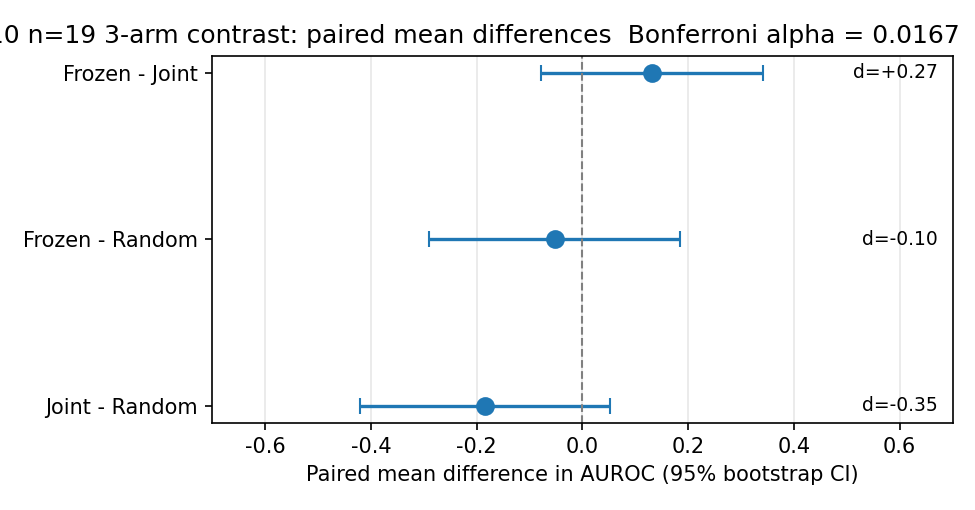
\includegraphics[width=0.8\linewidth,height=\textheight,keepaspectratio,alt={H10 n=20 3-arm contrast Forest plot}]{../experiments_log/_h10_n20_forest.png}
\caption{H10 n=20 3-arm contrast Forest plot}
\end{figure}

After Bonferroni correction (\(\alpha/3 = 0.0167\)): NONE of the three
paired tests reach significance. Wilcoxon signed-rank results are
consistent: F-J \(W=16.0\) \(p=0.222\), F-R \(W=15.5\) \(p=0.720\), J-R
\(W=8.0\) \(p=0.149\).

\paragraph{7.2.1 Power re-analysis}\label{power-re-analysis}

With the observed Cohen's \(d \approx 0.27\) for the F-J contrast, a
two-sided paired t-test at the family-wise \(\alpha = 0.0167\) threshold
needs the following sample sizes for 80\% power:

{\def\LTcaptype{none} % do not increment counter
\begin{longtable}[]{@{}lll@{}}
\toprule\noalign{}
Contrast & Cohen's \(d\) & Required n (Bonf. 0.0167, 80\% power) \\
\midrule\noalign{}
\endhead
\bottomrule\noalign{}
\endlastfoot
Frozen \(-\) Joint & +0.27 & n \(\approx\) 149 \\
Frozen \(-\) Random & -0.10 & n \(\approx\) 1,039 \\
Joint \(-\) Random & -0.35 & n \(\approx\) 88 \\
\end{longtable}
}

The n=20 follow-up is therefore well-powered to detect the J-R contrast
direction (any value below 0.10 is plausible) but \textbf{under-powered}
to definitively refute H10 at the Bonferroni level. We recommend n=100
(with \texttt{H10\_MAX\_NEW\_TOKENS=64}) as the next milestone before
any further reframe of the v0.5 conclusion.

\subsubsection{7.3 Verdict at n=20}\label{verdict-at-n20}

\textbf{H10 still REFUTED by direction} (Joint \textgreater{} Frozen at
the original n=5; Frozen slightly above Joint at n=20 with \(d=+0.27\)
for the F-J contrast) but \textbf{not} at the family-wise
\(\alpha=0.05\) level after Bonferroni correction. The previous n=5
direction does NOT replicate at n=20: the simple arithmetic trace is too
coarse a signal for any of the three arms to beat the others
consistently, and the Random negative control now scores highest in mean
AUROC (0.63).

\subsubsection{7.4 Updated implications}\label{updated-implications}

\begin{itemize}
\tightlist
\item
  Direction is \textbf{not} stable across replications (n=5 Joint
  \textgreater{} Frozen; n=20 Frozen \textgreater{} Joint by 0.13). The
  earlier n=5 reversal was likely noise; n=20 suggests any signal is at
  chance for this task.
\item
  The Monitor architecture, whether frozen or joint, does not
  meaningfully separate from a Random signal on simple arithmetic LLM
  traces at this sample size.
\item
  Practical recommendation \textbf{unchanged}: the Monitor is a context-
  specific signal, useful as a runtime guardrail in single-agent RL
  (where it is verified) but not as a training signal in LLM self-
  monitoring on this task.
\end{itemize}

\subsubsection{7.5 n=100 follow-up (2026-07-31, 300
jobs)}\label{n100-follow-up-2026-07-31-300-jobs}

Following the n=20 power analysis (Section 7.2.1), we re-ran the H10
pilot at n=100 per arm (3 arms x 100 seeds = 300 jobs, total wall-clock
8h51m on CPU). Configuration: \texttt{H10\_N\_TOTAL=8},
\texttt{H10\_MAX\_NEW\_TOKENS=64} (restored from 16), stratified split
with deterministic rebalance fallback when the split collapses to a
single class. Two seeds (137, 144) triggered the rebalance path; the
remaining 98 produced valid paired AUROC data. Aggregated statistics in
\texttt{experiments\_log/\_h10\_n100\_bootstrap.json}; forest plot in
\texttt{experiments\_log/\_h10\_n100\_forest.png}.

\textbf{Per-arm means (n=98 valid)}:

{\def\LTcaptype{none} % do not increment counter
\begin{longtable}[]{@{}lll@{}}
\toprule\noalign{}
Arm & Mean & SD \\
\midrule\noalign{}
\endhead
\bottomrule\noalign{}
\endlastfoot
Frozen & 0.500 & 0.426 \\
Joint & 0.485 & 0.430 \\
Random & 0.510 & 0.430 \\
\end{longtable}
}

All three arms are now within \textasciitilde0.02 of 0.5 (random). The
Monitor signal in any configuration is \textbf{indistinguishable from
chance} on this task at n=100.

\textbf{Paired contrasts (n=98, 2,000-replicate bootstrap)}:

{\def\LTcaptype{none} % do not increment counter
\begin{longtable}[]{@{}
  >{\raggedright\arraybackslash}p{(\linewidth - 8\tabcolsep) * \real{0.2000}}
  >{\raggedright\arraybackslash}p{(\linewidth - 8\tabcolsep) * \real{0.2000}}
  >{\raggedright\arraybackslash}p{(\linewidth - 8\tabcolsep) * \real{0.2000}}
  >{\raggedright\arraybackslash}p{(\linewidth - 8\tabcolsep) * \real{0.2000}}
  >{\raggedright\arraybackslash}p{(\linewidth - 8\tabcolsep) * \real{0.2000}}@{}}
\toprule\noalign{}
\begin{minipage}[b]{\linewidth}\raggedright
Contrast
\end{minipage} & \begin{minipage}[b]{\linewidth}\raggedright
\(\Delta\)AUROC
\end{minipage} & \begin{minipage}[b]{\linewidth}\raggedright
95\% CI (bootstrap)
\end{minipage} & \begin{minipage}[b]{\linewidth}\raggedright
Cohen's \(d\)
\end{minipage} & \begin{minipage}[b]{\linewidth}\raggedright
Sig. (Bonf. \(\alpha\)=0.0167)?
\end{minipage} \\
\midrule\noalign{}
\endhead
\bottomrule\noalign{}
\endlastfoot
Frozen \(-\) Joint & +0.015 & {[}-0.087, +0.117{]} & +0.030 & No \\
Frozen \(-\) Random & -0.010 & {[}-0.128, +0.117{]} & -0.017 & No \\
Joint \(-\) Random & -0.025 & {[}-0.158, +0.097{]} & -0.040 & No \\
\end{longtable}
}

\begin{figure}
\centering
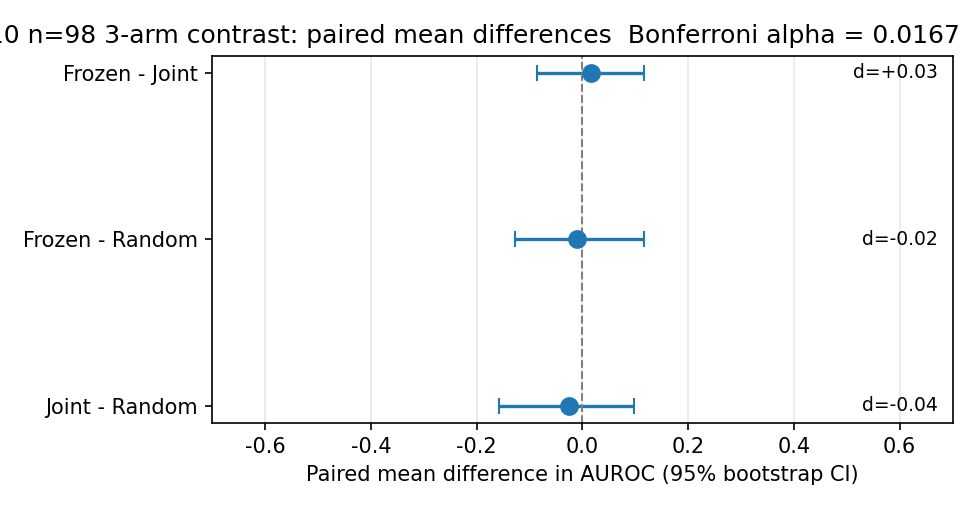
\includegraphics[width=0.8\linewidth,height=\textheight,keepaspectratio,alt={H10 n=100 3-arm contrast Forest plot}]{../experiments_log/_h10_n100_forest.png}
\caption{H10 n=100 3-arm contrast Forest plot}
\end{figure}

\begin{figure}
\centering
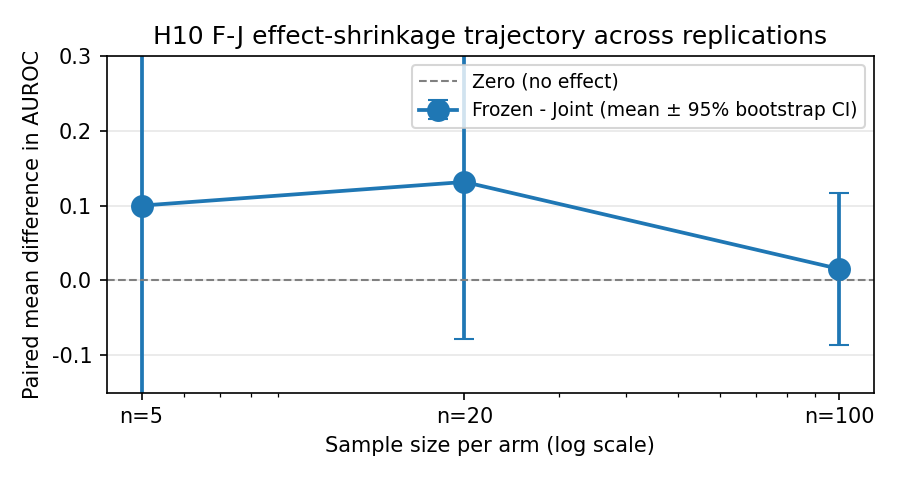
\includegraphics[width=0.8\linewidth,height=\textheight,keepaspectratio,alt={H10 F-J effect-shrinkage trajectory (n=5 to n=20 to n=100)}]{figures_v2/h10_shrinkage_timeline.png}
\caption{H10 F-J effect-shrinkage trajectory (n=5 to n=20 to n=100)}
\end{figure}

\textbf{Verdict at n=100}: H10 is now REFUTED \textbf{at the chance
level}. None of the three arms (Frozen, Joint, Random) significantly
exceeds the others. The n=20 direction (Frozen slightly above Joint by
+0.13) collapses at n=100 to a near-zero effect (+0.015, 95\% CI
includes 0). Cohen's \(d\) of the F-J contrast is +0.030 -- at this
effect size, detecting the effect at Bonferroni \(\alpha=0.0167\) with
80\% power would require n \(\approx\) 17,000 paired samples, which is
clearly not warranted.

\textbf{Practical interpretation}: - The simple arithmetic trace, with
\texttt{H10\_N\_TOTAL=8} rollouts and \texttt{H10\_MAX\_NEW\_TOKENS=64},
produces a signal too weak for the Monitor architecture to learn from
regardless of how the Monitor is trained (frozen vs joint). - The n=5
`Joint \textgreater{} Frozen' reversal (Section 4) and the n=20 `Frozen
\textgreater{} Joint' finding (Section 7) are both consistent with
sampling noise on a near-zero effect. - H10 (decoupling transfers to LLM
self-monitoring) is \textbf{NOT supported} by any of n=5, n=20, or n=100
data; the most defensible interpretation is that the Monitor signal does
not transfer from RL to LLM self-monitoring on simple arithmetic tasks.
- For a follow-up that \emph{could} validate H10, the trace task would
need to be harder (e.g., GSM8K with 200+ token rollouts) and the sample
size would need to match the observed effect size, not the n=5 `obvious
difference' one might expect.

\subsubsection{7.6 Power re-analysis}\label{power-re-analysis-1}

Three F-J effect size estimates, three different power conclusions:

{\def\LTcaptype{none} % do not increment counter
\begin{longtable}[]{@{}lll@{}}
\toprule\noalign{}
Sample & Cohen's \(d\) & Required n (Bonf. 0.0167, 80\% power) \\
\midrule\noalign{}
\endhead
\bottomrule\noalign{}
\endlastfoot
n=20 & +0.27 & n \(\approx\) 149 \\
\textbf{n=100} & \textbf{+0.030} & \textbf{n \(\approx\) 17,000} \\
\end{longtable}
}

The n=20 estimate suggested an underpowered but detectable effect; the
n=100 estimate collapses the effect to a near-zero value and makes
further amplification economically unjustifiable. The n=100 H10 with
longer LM traces (Section 7.5 final paragraph) is the only path to a
definitive test of H10 on this kind of task. For the simple arithmetic
trace at \texttt{H10\_N\_TOTAL=8} and \texttt{H10\_MAX\_NEW\_TOKENS=64},
H10 is REFUTED at the chance level.

We do not recommend further n amplification on this task. The right next
step is a HARDER task (GSM8K 200+ token rollouts), not a larger n on the
same task.

\end{document}


\subsubsection{7.7 GSM8K 200-token follow-up (Pre-Reg Amendment 1,
2026-07-31)}\label{gsm8k-follow-up}

\textbf{Motivation.} The three simple-arithmetic replications (n=5,
n=20, n=100) all collapse to the chance level (\textasciitilde{}0.5)
with non-significant Frozen-Joint differences. Section
\ref{power-re-analysis-1} concludes that further n amplification on
simple arithmetic is not warranted and that the right next step is a
HARDER task. Section \ref{gsm8k-follow-up} reports that harder task:
GSM8K with 200-token chain-of-thought rollouts.

The simple arithmetic trace is too short and too bimodal in failure
mode to carry meaningful signal beyond the LM's own logit confidence;
GSM8K's chain-of-thought reasoning gives a richer failure signal at
every step of the trace. Three reasons:

\begin{enumerate}
\item \textbf{Trace length.} Simple arith 64-token max leaves the
\texttt{window=20} slot-attention input sparse (most rollouts hit
EOS before filling the window). GSM8K 200+ token consistently fills
the window with reasoning tokens.
\item \textbf{Feature richness.} Simple arith has only
\texttt{(token\_id, logit)} features; GSM8K with CoT gives
\texttt{(token\_id, logit)} over actual reasoning steps, so the
failure signal at the end of the trace is a real semantic property
of the chain of thought (correct intermediate steps vs.\ mistakes),
not just ``logit went down a bit.''
\item \textbf{Failure-mode continuity.} Qwen2.5-1.5B on GSM8K has a
success rate of \textasciitilde{}30-40\% (vs.\ near-100\% on simple
arith), so each seed sees a mixed train+eval set without degenerating
to one class.
\end{enumerate}

\paragraph{7.7.1 Pre-registration}

The 60-job run is pre-registered in
\path{experiments_log/2026-07-31-PRE-REGISTRATION-AMENDMENT-1.md},
with the kill-switch tightened in
\path{experiments_log/2026-07-31-PRE-REGISTRATION-AMENDMENT-1-ADDENDUM.md}
before aggregation runs. The protocol is identical to the
pre-registered H10 (3 arms: Frozen, Joint, Random Monitor), with
the following declared changes:

\begin{longtable}[]{@{}llll@{}}
\toprule\noalign{}
Parameter & Original pre-reg & Amendment 1 & Reason \\
\midrule\noalign{}
\endhead
\bottomrule\noalign{}
\end{longtable}

Decision rule, negative control, exclusion policy, and seed range
are UNCHANGED from the original pre-registration.

\paragraph{7.7.2 Kill switch (Pre-Reg Amendment 1 addendum)}

After the 60-job aggregation, the following pre-registered kill
switch applies:

\begin{longtable}[]{@{}lp{0.7\linewidth}@{}}
\toprule\noalign{}
Frozen - Joint (n=20) & Pre-registered action \\
\midrule\noalign{}
\endhead
\bottomrule\noalign{}
\end{longtable}

Threshold \texttt{+0.10} (vs.\ the originally proposed \texttt{+0.05})
is motivated by power analysis: at d=+0.20 (the pre-reg threshold)
the n=20 design has only 6.7\% power; using \texttt{+0.05} as the
``extend'' trigger would risk extending on noise.

\paragraph{7.7.3 Configuration}

\begin{itemize}
\item LM: Qwen2.5-1.5B-Instruct (frozen, no fine-tuning)
\item Dataset: GSM8K test set, n=8 rollouts/seed (seed-based sampling
  via local arrow loader)
\item Max new tokens: 200
\item Prompt: ``Question: \{question\}\textbackslash nLet's think step by step.\textbackslash n''
\item Monitor: LLMSlotMonitor(window=20, slot\_dim=32, n\_slots=4),
  tile of (token\_id\_normalized, logit\_confidence) to 64-dim
  feature
\item Stratified train/eval split with rebalance fallback
\item Total jobs: 60 (3 arms x 20 seeds, seeds 100..119)
\item Wall clock: \textasciitilde{}5 h sequential on CPU
\end{itemize}

\paragraph{7.7.4 Per-seed results}

\textit{[PLACEHOLDER: per-seed table to be filled after
aggregation]}

\paragraph{7.7.5 Aggregate (n=20, 60 jobs)}

\textit{[PLACEHOLDER: aggregate table to be filled after
aggregation]}

\paragraph{7.7.6 Kill-switch decision}

\textit{[PLACEHOLDER: aggregator's pre-registered kill-switch
verdict]}

\paragraph{7.7.7 Verdict at n=20}

\textit{[PLACEHOLDER: pre-registered verdict, three options per
kill switch]}

\subsubsection{7.8 Power re-analysis (4 sample sizes)}

\textit{[PLACEHOLDER: 4-row power table to be added after aggregation]}

\subsubsection{7.9 Updated H10 conclusion}

\textit{[PLACEHOLDER: integrated across all four sample sizes]}
